\documentclass[10pt]{article}

\usepackage[paperwidth=30in,paperheight=40in,margin=0.42in]{geometry}
\usepackage[T1]{fontenc}
\usepackage{lmodern}
\usepackage{microtype}
\usepackage{amsmath,amssymb}
\usepackage{graphicx}
\usepackage{array}
\usepackage{enumitem}
\usepackage{xcolor}
\usepackage{tikz}
\usetikzlibrary{arrows.meta,positioning,calc,decorations.pathmorphing}
\usepackage{ragged2e}
\usepackage[hidelinks]{hyperref}

\renewcommand{\familydefault}{\sfdefault}

% Muted palette matched to the manually arranged PowerPoint poster.
\definecolor{PosterInk}{HTML}{23313A}
\definecolor{PosterSlate}{HTML}{496577}
\definecolor{PosterSage}{HTML}{658B70}
\definecolor{PosterClay}{HTML}{956B58}
\definecolor{PosterFog}{HTML}{EEF1F2}
\definecolor{PosterSand}{HTML}{F3F0EA}
\definecolor{PosterLine}{HTML}{CCD4D8}
\definecolor{PosterMuted}{HTML}{53616A}

\hypersetup{
  pdftitle={Recovering 3D Vibration Modes from Asynchronous Multi-View Videos},
  pdfauthor={Brian Song, Tianyi Zhang, Abe Davis},
  colorlinks=true,
  linkcolor=PosterSlate,
  urlcolor=PosterSlate
}

\graphicspath{{bush_spatial_modes_poster_final_assets/}%
  {docs/poster_drafts/bush_spatial_modes_poster_final_assets/}}

\pagestyle{empty}
\setlength{\parindent}{0pt}
\setlength{\parskip}{0.17em}
\setlist[itemize]{leftmargin=1.15em,itemsep=0.08em,topsep=0.10em}

\newcommand{\postersection}[3]{%
  \vspace{0.12in}%
  \noindent\colorbox{#3}{%
    \parbox{\dimexpr\linewidth-2\fboxsep\relax}{%
      \color{white}\bfseries\fontsize{31}{35}\selectfont
      \strut #1\hspace{0.20em}#2\strut}}%
  \vspace{0.07in}%
}

\newcommand{\postersubsection}[1]{%
  \vspace{0.07in}%
  {\bfseries\color{PosterInk}\fontsize{22}{26}\selectfont #1\par}%
  \vspace{0.01in}%
}

\newcommand{\equationbox}[2]{%
  \par\vspace{0.04in}%
  \noindent\fcolorbox{#1}{PosterFog}{%
    \parbox{\dimexpr\linewidth-2\fboxsep-2\fboxrule\relax}{%
      \centering\vspace{0.04in}%
      {\fontsize{17}{21}\selectfont$\displaystyle #2$\par}%
      \vspace{0.04in}}}%
  \par\vspace{0.04in}%
}

\newcommand{\notebox}[2]{%
  \par\vspace{0.04in}%
  \noindent\fcolorbox{#1}{PosterSand}{%
    \parbox{\dimexpr\linewidth-2\fboxsep-2\fboxrule\relax}{%
      \RaggedRight\vspace{0.04in}\textbf{#2}\vspace{0.04in}}}%
  \par\vspace{0.04in}%
}

\newcommand{\posterimage}[3]{%
  \begin{center}
    \includegraphics[width=\linewidth,height=#2,keepaspectratio]{#1}\par
    \vspace{0.01in}%
    {\color{PosterMuted}\fontsize{14}{17}\selectfont #3\par}
  \end{center}%
}

\newcommand{\pipelinebox}[4]{%
  \node[draw=#1,fill=#1!7,line width=1.5pt,rounded corners=3pt,
        align=center,text width=2.82in,minimum height=0.62in,#4] (#2)
        {\bfseries\fontsize{16}{19}\selectfont #3};%
}

\begin{document}
\RaggedRight
\color{PosterInk}
\fontsize{18}{22}\selectfont

% -----------------------------------------------------------------------------
% Full-width header and pipeline.
% -----------------------------------------------------------------------------
\begin{center}
  {\bfseries\fontsize{70}{75}\selectfont
    Recovering 3D Vibration Modes from\\[-0.03in]
    Asynchronous Multi-View Videos\par}
  \vspace{0.06in}
  {\color{PosterSlate}\fontsize{27}{32}\selectfont
    Brian Song, Tianyi Zhang, Abe Davis\par}
\end{center}

\vspace{0.09in}
\noindent\colorbox{PosterSand}{%
  \parbox{\dimexpr\linewidth-2\fboxsep\relax}{%
    \centering\fontsize{20}{25}\selectfont
    \textbf{Goal.} Use one mobile phone to scan a static scene and record
    vibration from several fixed viewpoints at different times. Recover a
    view-consistent, high-detail 3D Gaussian model and spatial vibration fields
    without synchronized cameras.}}
\vspace{0.08in}

\begin{center}
  {\bfseries\color{PosterSlate}\fontsize{21}{25}\selectfont
    End-to-end pipeline\par}
  \vspace{0.02in}
  \begin{tikzpicture}[x=1in,y=1in,>=Latex]
    \pipelinebox{PosterSlate}{capture}{1. Sweep + fixed videos}{at={(1.46,0)}}
    \pipelinebox{PosterSlate}{colmap}{2. Joint COLMAP}{at={(5.00,0)}}
    \pipelinebox{PosterSage}{static}{3. Static 3DGS}{at={(8.54,0)}}
    \pipelinebox{PosterClay}{flow}{4. Flow + Fourier modes}{at={(12.08,0)}}
    \pipelinebox{PosterSage}{topology}{5. Pixel--Gaussian topology}{at={(15.62,0)}}
    \pipelinebox{PosterClay}{phase}{6. View phase sync}{at={(19.16,0)}}
    \pipelinebox{PosterSlate}{solve}{7. Local 3D solve}{at={(22.70,0)}}
    \pipelinebox{PosterSage}{fill}{8. Motion fill}{at={(26.24,0)}}
    \draw[->,PosterMuted,line width=1.5pt] (capture) -- (colmap);
    \draw[->,PosterMuted,line width=1.5pt] (colmap) -- (static);
    \draw[->,PosterMuted,line width=1.5pt] (static) -- (flow);
    \draw[->,PosterMuted,line width=1.5pt] (flow) -- (topology);
    \draw[->,PosterMuted,line width=1.5pt] (topology) -- (phase);
    \draw[->,PosterMuted,line width=1.5pt] (phase) -- (solve);
    \draw[->,PosterMuted,line width=1.5pt] (solve) -- (fill);
  \end{tikzpicture}
  \vspace{0.01in}

  {\color{PosterMuted}\fontsize{15}{18}\selectfont
    Output: completed complex spatial fields
    $\boldsymbol\phi_k\in\mathbb C^{G\times3}$.\par}
\end{center}

\vspace{0.02in}

% -----------------------------------------------------------------------------
% Explicit three-column layout. This mirrors the approved PowerPoint rather
% than relying on automatic multi-column flow. Phase synchronization begins in
% column two and intentionally continues at the top of column three.
% -----------------------------------------------------------------------------
\noindent
\begin{minipage}[t]{0.326\textwidth}
\vspace{0pt}

\postersection{1.}{3D Gaussian Splatting}{PosterSlate}

3D Gaussian Splatting (3DGS) represents a scene with explicit, oriented,
semi-transparent ellipsoids. Gaussian $g$ stores

\equationbox{PosterSlate}{
  \mathcal G_g=(\boldsymbol\mu_g,\boldsymbol\Sigma_g,o_g,\mathbf c_g).
}

Here $\boldsymbol\mu_g\in\mathbb R^3$ is its center,
$\boldsymbol\Sigma_g$ its covariance, $o_g$ opacity, and $\mathbf c_g$
appearance. In view $v$, its opacity at pixel $p$ is

\[
  a_{vpg}=o_g\exp\!\left[-\frac12
  (p-\mathbf m_{vg})^\top
  (\boldsymbol\Sigma^{2D}_{vg})^{-1}(p-\mathbf m_{vg})\right].
\]

A calibrated camera projects and depth-sorts the Gaussians. Front-to-back
alpha compositing gives

\equationbox{PosterSlate}{
  \widehat{\mathbf C}_v(p)=\sum_g T_{vpg}a_{vpg}\mathbf c_g,
  \qquad
  T_{vpg}=\prod_{h\prec g}(1-a_{vph}).
}

The sweep video trains one canonical foreground/background 3DGS. Its explicit
centers become the 3D nodes on which vibration modes are recovered.

\begin{center}
  \begin{minipage}[t]{0.57\linewidth}
    
\includegraphics[width=\linewidth,height=3.15in,keepaspectratio]
      {3dgs_schematic.png}
  \end{minipage}\hfill
  \begin{minipage}[t]{0.39\linewidth}
    
\includegraphics[width=\linewidth,height=3.15in,keepaspectratio]
      {3dgs_scene.png}
  \end{minipage}
  \par\vspace{0.01in}
  {\color{PosterMuted}\fontsize{14}{17}\selectfont
    Oriented Gaussian primitives and an explicit reconstructed scene.\par}
\end{center}

\postersection{2.}{Why Modal Analysis?}{PosterSage}

\postersubsection{A. What is modal analysis?}

A vibrating object is a coupled mechanical system with many physical degrees
of freedom:

\equationbox{PosterSage}{
  \mathbf M\ddot{\mathbf u}+\mathbf C\dot{\mathbf u}
  +\mathbf K\mathbf u=\mathbf f,
  \qquad
  \mathbf K\boldsymbol\phi_k
  =\omega_k^2\mathbf M\boldsymbol\phi_k.
}

Modal analysis describes its displacement with a small set of coherent spatial
patterns:

\equationbox{PosterSage}{
  \mathbf u(t)\approx\boldsymbol\Phi\mathbf q(t)
  =\sum_{k=1}^{K}\boldsymbol\phi_k q_k(t),
  \qquad K\ll N.
}

Each $\boldsymbol\phi_k$ is a spatial \emph{mode shape}; $q_k(t)$ is its
time-varying modal coordinate. For small linear vibration, the modes
approximately decouple and behave like independent damped oscillators. A
camera observes their projected motion,

\[
  \mathbf d_v(t)\approx\mathbf J_v\mathbf u(t)
  =\sum_k(\mathbf J_v\boldsymbol\phi_k)q_k(t).
\]

\begin{center}
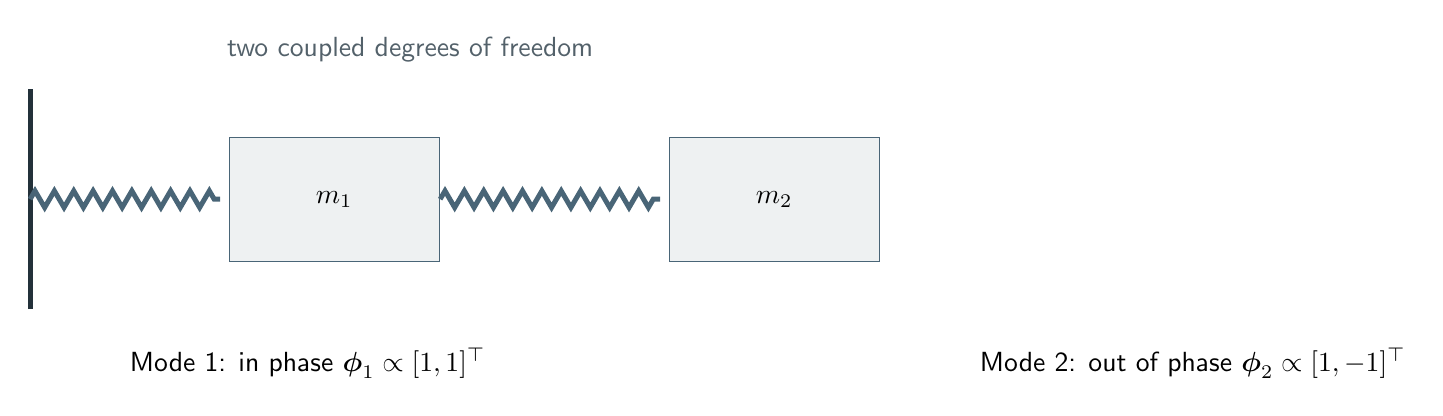
\begin{tikzpicture}[x=1in,y=1in,>=Latex]
  \draw[PosterInk,line width=1.8pt] (0.2,0.35) -- (0.2,1.45);
  \draw[PosterSlate,line width=1.8pt,decorate,
        decoration={zigzag,segment length=7pt,amplitude=3pt}]
        (0.2,0.90) -- (1.15,0.90);
  \node[draw=PosterSlate,fill=PosterFog,minimum width=1.05in,
        minimum height=0.62in] (m1) at (1.72,0.90) {$m_1$};
  \draw[PosterSlate,line width=1.8pt,decorate,
        decoration={zigzag,segment length=7pt,amplitude=3pt}]
        (2.25,0.90) -- (3.35,0.90);
  \node[draw=PosterSlate,fill=PosterFog,minimum width=1.05in,
        minimum height=0.62in] (m2) at (3.92,0.90) {$m_2$};
  \node[PosterMuted] at (2.1,1.65) {two coupled degrees of freedom};
  \node[anchor=west] at (0.65,0.08)
    {Mode 1: in phase $\boldsymbol\phi_1\propto[1,1]^\top$};
  \node[anchor=west] at (4.90,0.08)
    {Mode 2: out of phase $\boldsymbol\phi_2\propto[1,-1]^\top$};
\end{tikzpicture}
\end{center}

\postersubsection{B. Why use frequency-domain video?}

Following Davis et al., we treat the displacement of every tracked pixel as a
degree of freedom. Time-domain motion mixes modes; the temporal Fourier
transform separates responses by natural frequency. We use a mean-removed,
Hann-windowed exact DFT:

\equationbox{PosterSage}{
  \begin{aligned}
    \widehat{\mathbf d}_{v,p}(f)
    &=\sum_{n=0}^{T_v-1}h_n
      (\mathbf d_{v,p}[n]-\bar{\mathbf d}_{v,p})
      e^{-2\pi i f n/F_v},\\
    h_n&=\tfrac12\!\left(1-\cos\tfrac{2\pi n}{T_v-1}\right).
  \end{aligned}
}

Near a resonant frequency $f_k$, one mode often dominates:

\[
  \widehat{\mathbf d}_v(f_k)\propto
  \mathbf J_v\boldsymbol\phi_k.
\]

Strong, camera-visible resonances therefore provide a compact set of
representative modes. Each complex Fourier slice preserves projected
displacement magnitude and relative phase.

\begin{center}
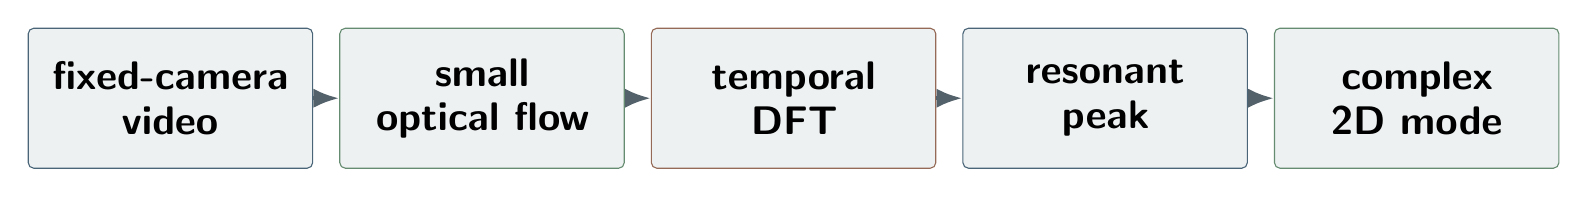
\begin{tikzpicture}[node distance=0.13in,>=Latex]
  \tikzset{stage/.style={draw=PosterSlate,fill=PosterFog,rounded corners=2pt,
    minimum height=0.70in,text width=1.33in,align=center,
    font=\bfseries\fontsize{14}{16}\selectfont}}
  \node[stage] (video) {fixed-camera\\video};
  \node[stage,right=of video,draw=PosterSage] (flow2d) {small\\optical flow};
  \node[stage,right=of flow2d,draw=PosterClay] (fft) {temporal\\DFT};
  \node[stage,right=of fft] (peak) {resonant\\peak};
  \node[stage,right=of peak,draw=PosterSage] (mode2d) {complex\\2D mode};
  \draw[->,PosterMuted,line width=1.4pt] (video) -- (flow2d);
  \draw[->,PosterMuted,line width=1.4pt] (flow2d) -- (fft);
  \draw[->,PosterMuted,line width=1.4pt] (fft) -- (peak);
  \draw[->,PosterMuted,line width=1.4pt] (peak) -- (mode2d);
\end{tikzpicture}
\end{center}

\posterimage{bush_2d_modal_modes.png}{4.20in}{%
  One Bush reference frame, modal amplitude, and complex $u/v$ phase images.}

\posterimage{bush_power_spectrum.png}{2.35in}{%
  Global power spectrum; selected peaks supply candidate modal frequencies.}

\end{minipage}
\hfill
\begin{minipage}[t]{0.326\textwidth}
\vspace{0pt}

\postersection{3.}{Why Asynchronous Multi-View Is Different}{PosterClay}

Synchronized cameras observe the same moving surface at the same instant. A
single phone can revisit several viewpoints, but each recording begins at an
unknown time; their optical flows cannot be matched frame by frame.

\begin{center}
\begin{tikzpicture}[x=1in,y=1in,>=Latex]
  \node[draw=PosterSage,fill=PosterSage!10,ellipse,minimum width=1.25in,
        minimum height=0.70in,align=center] (object) at (4.55,1.52)
        {same\\object};
  \node[draw=PosterSlate,fill=PosterFog,minimum width=0.78in,
        minimum height=0.62in] (v1) at (1.90,2.58) {};
  \node[draw=PosterSlate,fill=PosterFog,minimum width=0.78in,
        minimum height=0.62in] (v2) at (1.90,0.45) {};
  \node[draw=PosterSlate,fill=PosterFog,minimum width=0.78in,
        minimum height=0.62in] (v3) at (7.20,1.52) {};
  \draw[dashed,PosterLine,line width=1.4pt] (v1) -- (object);
  \draw[dashed,PosterLine,line width=1.4pt] (v2) -- (object);
  \draw[dashed,PosterLine,line width=1.4pt] (v3) -- (object);
  \node[align=center,PosterMuted] at (1.90,1.87)
    {video 1\\unknown start $\tau_1$};
  \node[align=center,PosterMuted] at (1.90,-0.22)
    {video 2\\unknown start $\tau_2$};
  \node[align=center,PosterMuted] at (7.20,0.82)
    {video 3\\unknown start $\tau_3$};
  \node[draw=PosterClay,fill=PosterSand,align=center,text width=2.55in]
    at (4.55,0.10)
    {same resonant frequency $f_k$\\different complex phase};
\end{tikzpicture}
\end{center}

\notebox{PosterClay}{Frequency-domain consistency assumption. If geometry,
boundary conditions, and material properties remain fixed, the same natural
frequency represents the same underlying 3D spatial mode. Each recording may
observe it with a different complex phase.}

\postersubsection{Working assumptions}

\begin{itemize}
  \item A static sweep defines one canonical rest geometry.
  \item Fixed reference cameras are calibrated in that coordinate system.
  \item Vibrations remain small enough for camera and modal linearization.
  \item Natural frequencies remain stable across recordings.
\end{itemize}

\postersection{4.}{Solving Shared 3D Modes}{PosterSlate}

\postersubsection{A. Shared canonical scene}

We place sampled sweep frames and one reference image from every fixed view in
the same COLMAP reconstruction. Registered sweep views train the canonical
foreground/background 3DGS; fixed-view intrinsics and poses are retained for
modal projection.

\begin{center}
  
\includegraphics[width=0.63\linewidth,height=3.10in,keepaspectratio]
    {bush_canonical_cameras.jpg}\par
  \vspace{0.02in}
  
\includegraphics[width=0.31\linewidth,height=1.65in,keepaspectratio]
    {bush_view1.png}\hfill
  
\includegraphics[width=0.31\linewidth,height=1.65in,keepaspectratio]
    {bush_view2.png}\hfill
  
\includegraphics[width=0.31\linewidth,height=1.65in,keepaspectratio]
    {bush_view3.png}\par
  {\color{PosterMuted}\fontsize{14}{17}\selectfont
    One canonical Gaussian scene and three calibrated fixed views.\par}
\end{center}

\postersubsection{B. Pixel--Gaussian observation topology}

For foreground pixel $p$, rendered depth unprojects a canonical surface point

\[
  \mathbf X_{v,p}=\pi_v^{-1}(p,\widehat D_v(p)).
\]

We preselect nearby Gaussians and rank them by anisotropic density and opacity:

\equationbox{PosterSage}{
  s_{vpg}=o_g\exp\!\left[-\frac12
  (\mathbf X_{v,p}-\boldsymbol\mu_g)^\top
  \boldsymbol\Sigma_g^{-1}
  (\mathbf X_{v,p}-\boldsymbol\mu_g)\right].
}

\[
  w_{vpg}=\frac{s_{vpg}}
  {\sum_{h\in\mathcal C(v,p)}s_{vph}}.
\]

This mode-independent topology connects each complex 2D measurement to a small
set of plausible visible foreground Gaussians. Camera calibration supplies

\[
  \mathbf J_{v,g}=
  \frac{\partial\pi_v(\boldsymbol\mu_g)}
       {\partial\boldsymbol\mu_g}\in\mathbb R^{2\times3}.
\]

\postersubsection{C. Phase synchronization without synchronized time}

At frequency $f_k$, view $v$ observes a complex 2D displacement
$\mathbf y_{v,k,p}=\widehat{\mathbf d}_{v,p}(f_k)$. We use a phase-only
cross-view model:

\equationbox{PosterClay}{
  \mathbf y_{v,k,p}\approx
  \alpha_{v,k}\mathbf J_{v,g}\boldsymbol\phi_{k,g},
  \qquad
  \alpha_{v,k}=e^{i\theta_{v,k}}.
}

Define inverse phase $\beta_{v,k}=\alpha_{v,k}^{-1}$. For a Gaussian shared
by several cameras, weighted equations stack as

\equationbox{PosterClay}{
  \mathcal A_g\boldsymbol\phi_{k,g}
  =\mathcal B_{g,k}\boldsymbol\beta_k.
}

\end{minipage}
\hfill
\begin{minipage}[t]{0.326\textwidth}
\vspace{0pt}

\postersubsection{C. Phase synchronization (continued)}

The columns of $\mathcal B_{g,k}$ place each view's measured complex flow in
its view block. Let $\mathbf N_g$ span the left null space of the stacked
projection Jacobian $\mathcal A_g$:

\equationbox{PosterClay}{
  \mathbf N_g^H\mathcal A_g=0
  \quad\Longrightarrow\quad
  \mathbf N_g^H\mathcal B_{g,k}\boldsymbol\beta_k=0.
}

The unknown 3D vector is now eliminated. We aggregate shared Gaussians and
solve only the relative phases:

\equationbox{PosterClay}{
  \begin{aligned}
    \boldsymbol\beta_k^\star
    &=\underset{\substack{|\beta_{v,k}|=1\\\beta_{1,k}=1}}
      {\arg\min}\;
      \sum_{g\in\mathcal G_{\rm shared}}\\[-0.08in]
    &\hspace{0.55in}
      \left\|\mathbf N_g^H\mathcal B_{g,k}
      \boldsymbol\beta_k\right\|_2^2.
  \end{aligned}
}

The gauge $\beta_{1,k}=1$ fixes arbitrary global phase. Aligned observations
are $\widetilde{\mathbf y}_{v,k,p}=\beta_{v,k}^\star\mathbf y_{v,k,p}$.

\notebox{PosterClay}{Interpretation. The left-null projection removes the
unknown 3D displacement from phase synchronization. It asks whether the
differently phased 2D observations could arise from one common 3D motion.}

\postersubsection{D. Spatial structure, local solve, and completion}

Mutual-KNN edges are built between observed foreground Gaussians. Edges that
cross strong Gaussian-color or rendered-depth discontinuities are removed;
each remaining connected component defines a local first-order rigid region.

For component $c$, a complex infinitesimal rigid twist
$\boldsymbol\xi_{k,c}=[\mathbf t_{k,c};\boldsymbol\omega_{k,c}]
\in\mathbb C^6$ gives

\equationbox{PosterSlate}{
  \mathbf H_{c,g}=
  \begin{bmatrix}\mathbf I_3&
  -[\boldsymbol\mu_g-\bar{\boldsymbol\mu}_c]_{\times}
  \end{bmatrix},
  \qquad
  \boldsymbol\phi_{k,g}=\mathbf H_{c,g}\boldsymbol\xi_{k,c}.
}

We recover its twist by matching projections to all aligned 2D observations:

\equationbox{PosterSlate}{
  \begin{aligned}
    \boldsymbol\xi_{k,c}^{\star}
    &=\underset{\boldsymbol\xi\in\mathbb C^6}{\arg\min}
      \sum_{(v,p,g)\in\mathcal O_c}w_{vpg}\\[-0.08in]
    &\hspace{0.50in}
      \left\|\mathbf J_{v,g}\mathbf H_{c,g}\boldsymbol\xi
      -\widetilde{\mathbf y}_{v,k,p}\right\|_2^2.
  \end{aligned}
}

\posterimage{bush_rigid_components.png}{5.10in}{%
  Observed Gaussian graph colored by local rigid component.}

A separate all-foreground graph propagates trusted observed motion into
compatible unobserved Gaussians. With trusted seeds held fixed, motion fill is
a harmonic extension:

\equationbox{PosterSage}{
  \begin{aligned}
    \min_{\boldsymbol\phi_k}\;&
      \sum_{(g,h)\in\mathcal E_{\rm fill}}
      \eta_{gh}\|\boldsymbol\phi_{k,g}
      -\boldsymbol\phi_{k,h}\|_2^2,\\
    &\eta_{gh}=\frac{1}{\|\boldsymbol\mu_g-\boldsymbol\mu_h\|+\epsilon},
      \qquad
      \boldsymbol\phi_{k,g}=\boldsymbol\phi^{\rm seed}_{k,g}
      \ (g\in\mathcal S).
  \end{aligned}
}

The result is one complex 3D displacement vector per foreground Gaussian:

\[
  \boldsymbol\phi_k\in\mathbb C^{G\times3},
  \qquad
  \Delta\boldsymbol\mu_g(\theta)
  =\operatorname{Re}\!\left(e^{i\theta}\boldsymbol\phi_{k,g}\right).
\]

\posterimage{bush_modal_comparison.png}{3.70in}{%
  Top: observed 2D modal images. Bottom: projections of the recovered 3D mode.}

Projecting the same recovered 3D mode into all three cameras produces similar
spatial and phase patterns to the observed modal images. This cross-view
agreement indicates that one shared 3D field explains the visible vibration.

\posterimage{bush_viser_viewer.png}{4.05in}{%
  Interactive Viser view of a recovered Bush spatial mode.}

\notebox{PosterSlate}{Current interpretation. The outputs are evidence-driven,
spatially coherent complex displacement fields. They are not yet mass- and
stiffness-normalized structural eigenmodes.}

\end{minipage}

\end{document}
